\section{Дубликатный маджонг}

\begin{additional}

В этом разделе описаны правила \textit{дубликатного} риичи-маджонга. В этой разновидности игры игроки на нескольких столах играют один и тот же расклад, чтобы потом выяснить, кто сыграл лучше.

\subsection{Начальная расстановка тайлов и порядок игры}

В дубликатном риичи-маджонге стартовые руки и стены выглядят следующим образом:

\begin{itemize}
	\item 4 стартовые руки по 13 тайлов,
	\item 4 стены по 18 тайлов каждая,
	\item мертвая стена из 12 тайлов.
\end{itemize}

\begin{figure}[H]
	\centering
	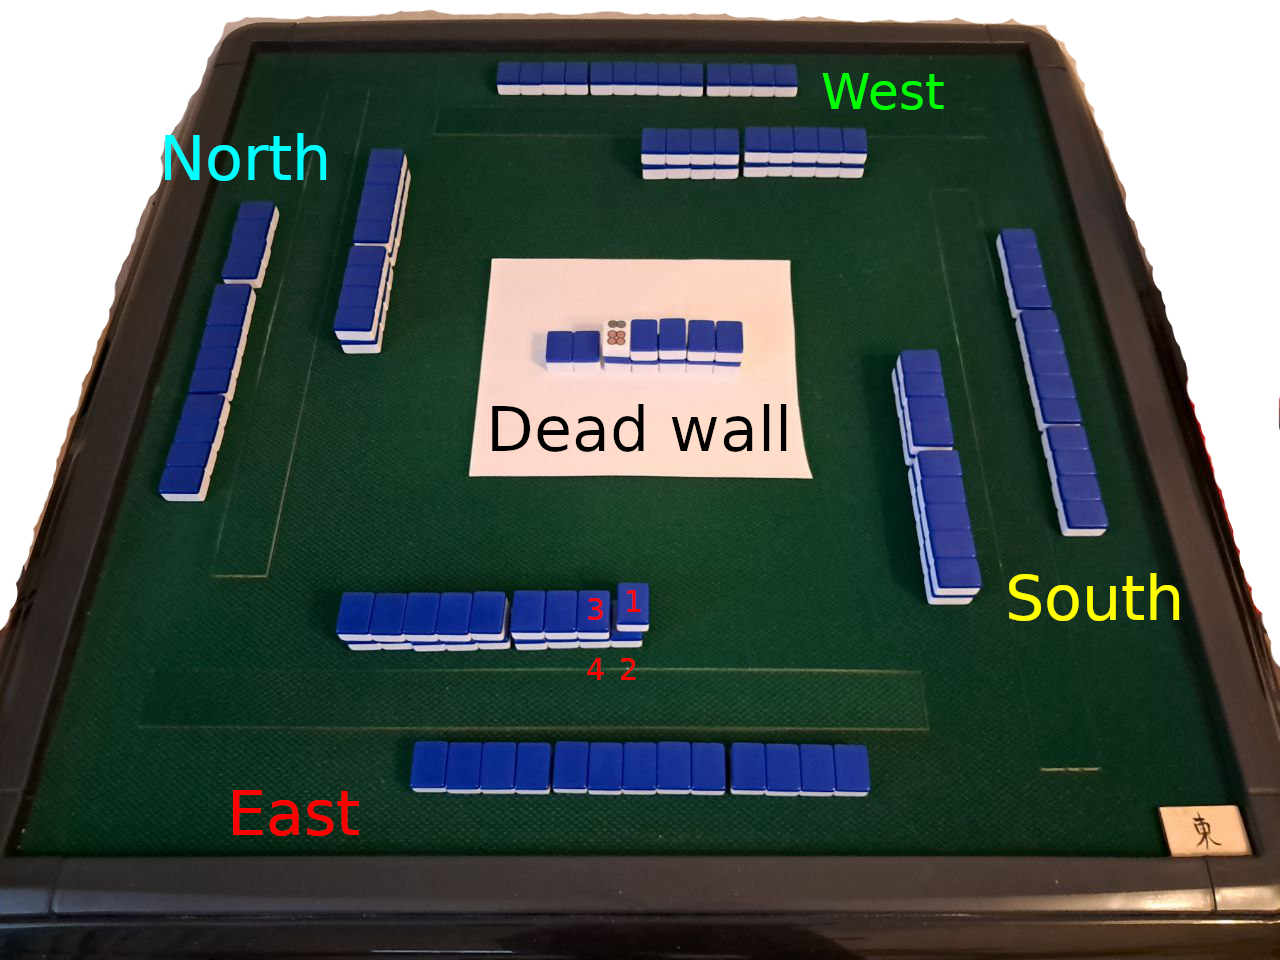
\includegraphics[width=8cm]{img/duplicate_start.png}
	\caption{Начальная расстановка тайлов для игры в дубликатный риичи-маджонг}
\end{figure}

\textit{В обычном риичи-маджонге при отсутствии объявлений игроки, сидящие на востоке и юге, возьмут по 18 тайлов, а игроки на западе и севере~--- по 17. Это число может меняться в случае объявления чи, понов и канов.}

В дубликатной версии у каждого игрока есть своя стена размером в 18 тайлов. Игроки всегда берут тайлы \textbf{из своей стены}, как после обычного взятия, так и в случае взятия тайла замены после кана. На картинке выше можно видеть пример стартовой расстановки, для игрока на востоке подписано, какой тайл он берет первым, вторым, третьим и четвертым.

Если игрок не может взять тайл со своей стены~--- раздача заканчивается вничью. В этом случае предыдущие взятие и сброс являются хотеем/хайтеем. Также, если в своей стене не осталось тайлов, нельзя объявить кан.

Мертвая стена имеет размер 12 тайлов. Из них два тайла вообще никак не участвуют в игре, а оставшиеся 10 являются индикаторами дор и урадор.

\subsection{Описание ханчана}

Каждый ханчан в дубликатной версии состоит из 12 раундов, обозначающихся от East 1 до West 4. Повторов дилера нет. На каждом столе в турнире эти раунды могут играться в произвольном порядке, но все 12 должны быть сыграны.

\textit{Мотивация выбрать 12 раундов происходит от того, что в среднем ханчан в риичи-маджонг длится чуть меньше 11 раундов, в зависимости от количество повторов дилеров, а также от того, что игра должна быть сбалансирована, т.е. каждый игрок одинаковое число раз должен побывать каждым ветром в игре.}

Пример. Пусть в турнире участвуют 24 человека. Тогда последовательность сыгранных раздач в ханчане за разными столами может выглядеть так:

\begin{itemize}
	\item 1 стол: E1, E2, E3, E4, S1, S2, S3, S4, W1, W2, W3, W4.
	\item 2 стол: E3, E4, S1, S2, S3, S4, W1, W2, W3, W4, E1, E2.
	\item 3 стол: S1, S2, S3, S4, W1, W2, W3, W4, E1, E2, E3, E4.
	\item 4 стол: S3, S4, W1, W2, W3, W4, E1, E2, E3, E4, S1, S2.
	\item 5 стол: W1, W2, W3, W4, E1, E2, E3, E4, S1, S2, S3, S4.
	\item 6 стол: W3, W4, E1, E2, E3, E4, S1, S2, S3, S4, W1, W2.
\end{itemize}

Для каждого игрока выделяется его стартовый ветер. Это тот ветер, на котором он играет раздачи E1, S1, W1. Он определяет, какой ветер будет у игрока во всех остальных раздачах.

Пример. Пусть стартовый ветер игрока~--- север, и он сидит на 6 столе в схеме, указанной выше. Тогда в первой его раздаче (W3) он будет сидеть на юге, во второй раздаче (W4)~--- на востоке, в третьей раздаче (E1)~--- на севере, в четвертой (E2)~--- на западе, и т.д.

\subsection{Итоги раздач и подсчет очков}

По завершении каждой раздачи ее итог (кто сколько очков заработал или потерял) записывается в протокол. В случае, если на столе осталась риичи-палочка, каждый игрок плюсует себе 250 очков за каждую палочку. Смысл этого таков~--- палочка, оставшаяся на столе, в обычном риичи-маджонге переходит в следующую раздачу, здесь же каждая раздача должна начинаться в одинаковых условиях, поэтому каждая палочка на столе делится поровну между игроками.

Подсчет очков для конкретного игрока за конкретную раздачу происходит следующим образом. Берутся результаты всех игроков, сидевших за этой раздачей на одном и том же стартовом ветре. Считается среднее этих результатов. Результат для игрока~--- это разница между его результатом и средним результатом.

Пример. Пусть в турнире участвует 24 человека, т.е. играется 6 столов. Пусть 6 игроков, стартовавших раздачу на одном и том же стартовом ветре, закончили ее с такими результатами: -2000, 0, 2000, 2000, 2600, 8000. Среднее этих результатов равно 2100. Таким образом, отклонения от среднего для этих 6 игроков равны -4100, -2100, -100, -100, 500, 5900.

Для каждой из 12 раздач такие отклонения от среднего суммируются и формируют итоговый результат игрока в ханчане. А результат в турнире~--- это сумма результатов во всех его ханчанах.

Возможен также маппинг отклонений от среднего в другую шкалу: к примеру, отклонение от 0 до 400 считать как 0 очков, от 400 до 900~--- как 1 очко, от 900 до 1500~--- как 2, и т.д.

\subsection{Порядок проведения игр}

Перед каждым ханчаном организаторы турнира должны подготовить 12 раскладов и пронумеровать их от East 1 до West 4. На рубашку каждого тайла необходимо наклеить стикер, обозначающий, где этот тайл должен лежать в стене.

Рекомендуется использовать маркеры разных цветов, например так:

\begin{itemize}
	\item тайлы востока~--- красный,
	\item тайлы востока~--- желтый,
	\item тайлы востока~--- зеленый,
	\item тайлы востока~--- синий,
	\item тайлы мертвой стены~--- черный.
\end{itemize}

Цвет маркеров не принципиален, главное, чтобы цвета были различимы между собой, и игроки знали и понимали, какой цвет что означает.

Далее,

\begin{itemize}
	\item стартовые руки обозначаются как ``---'' (порядок тайлов в стартовых руках не важен),
	\item тайлы стен игроков обозначаются числами от 1 до 18 (эти числа обозначают порядок взятия), 
	\item тайлы мертвой стены обозначаются числами от 1 до 12 (числа от 1 до 5 обозначают доры, где тайл 1 перевернут на старте игры, 6 и 7~--- не участвуют в игре, от 8 до 12~--- урадоры, где 8 лежит под 1, 9 под 2, и т.д.).
\end{itemize}

Около чисел 6 и 9 необходимо ставить точку, чтобы их не перепутать.

Обозначения могут быть и другими, главное, чтобы было понятно, где какой тайл должен находиться в стартовом раскладе. Альтернативные обозначения приведены на следующей схеме:

\begin{figure}[H]
	\centering
	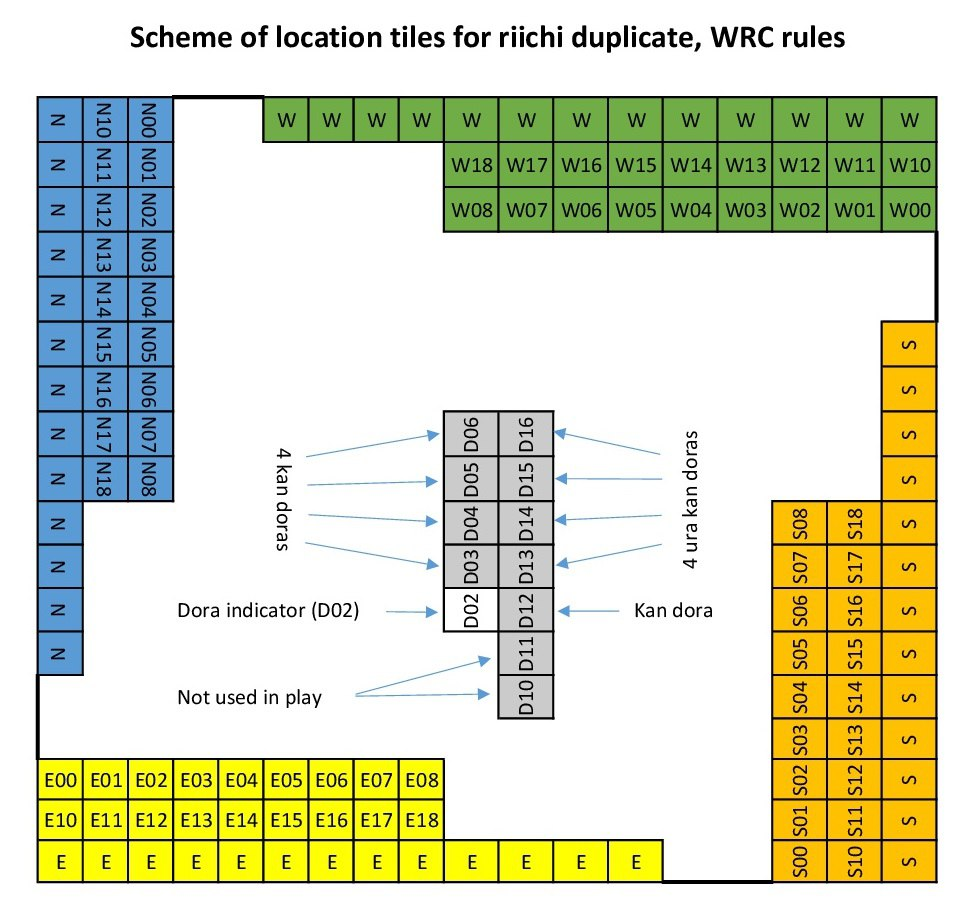
\includegraphics[width=8cm]{img/duplicate_marks.jpg}
	\caption{Пример обозначения тайлов для игры в дубликатный риичи-маджонг}
\end{figure}

Каждая раздача ставится на переносную доску. Организаторы приносят игрокам очередную раздачу, игроки ее играют, записывают результат и возвращают тайлы в стартовое положение согласно маркировкам на стикерах. После этого организаторы забирают доску с раздачей, и в будущем она отправится на другой стол, где ее разыграют другие игроки.

\end{additional}
